\section{Background and motivation}
\label{sec:motivation}

Injection remains among the most damaging and persistent classes of software
vulnerability. This section surveys the breadth of the problem beyond its most
familiar members, its measured prevalence and cost, and why the very machinery
built to contain it has itself become a recurring source of vulnerabilities:
the motivation for the structural approach this thesis evaluates.

\subsection{A wider family of embedding hazards}
\label{sec:bg:hazards}

SQL injection and XSS are only the most familiar members
of a much larger family that share the boundary-crossing cause of \cref{sec:intro}.
The same failure recurs across many more language pairs than those two,
and produces symptoms well beyond information disclosure.

Several are, like SQL injection, outright remote compromises.
In the 2021 Log4Shell vulnerability,
a \verb|${jndi:...}| sequence appearing anywhere in a logged string
was expanded by Log4j's message interpolation into a remote lookup
that loaded and executed attacker-supplied code~\cite{cve2021log4shell}.
Command injection arises when user input reaches a shell without proper quoting,
so that metacharacters such as \verb|;| or \verb|&|
break out of the intended single argument~\cite{owasp_cmdinjection}.
Spreadsheet formula injection turns exported data into code:
a field beginning with \verb|=| is re-interpreted as a formula
when a CSV export is opened in a spreadsheet,
as in an Azure activity-log entry
that executed on an administrator's machine on download~\cite{gietzen18csv}.
Server-side template injection embeds user input into a template
instead of passing it as data,
letting an expression such as \verb|{{7*7}}| reach the template engine
and frequently the whole server~\cite{portswigger_ssti},
while the analogous client-side attack
breaks out of the AngularJS expression sandbox
to run arbitrary JavaScript~\cite{peguero16angular}.
Even purpose-built defenses are not immune:
the DOMPurify sanitizer has been bypassed by \emph{mutation} XSS,
in which the browser's own parser rewrites already-sanitized markup
back into an executable form~\cite{heyes20mxss}.

Other members corrupt data or deny service rather than disclose it.
YAML's implicit typing silently coerces values,
so a list entry \verb|NO|, a country code, parses as the boolean false,
the widely cited ``Norway problem''~\cite{oconnor23yaml}.
A regular expression with nested quantifiers
fed adversarial input backtracks catastrophically and hangs the program,
a regular-expression denial of service~\cite{owasp_redos};
and the XML ``billion laughs'' attack
expands a kilobyte of nested entity definitions into gigabytes,
exhausting memory during parsing~\cite{sullivan09xml}.

The maintainability face of the same problem
is the leaning toothpick syndrome,
and history shows that ad-hoc syntactic fixes tend to backfire:
PHP's \verb|magic_quotes| feature auto-escaped quotes in request data
to forestall injection,
but did so inconsistently, invited double-escaping bugs,
and was eventually deprecated~\cite{php_magicquotes}.
What unites the largest of these cases is structural:
content meant to be inert data is read as syntax
because a bracket or quote within it escapes its intended region.
That is exactly the failure a matcher-balance discipline is built to resist,
and because it recurs across the injection and markup attacks above
rather than in any single language pair,
one structural discipline can address the breakout-based members at once---as
distinct from the execution and algorithmic members (template evaluation, ReDoS,
entity expansion) it cannot.


\subsection{The prevalence and cost of injection failures}
\label{sec:bg:prevalence}

These failures are neither rare nor fading.
Injection has appeared in every edition of the OWASP Top~10
web application security risks since 2010,
and since the 2021 edition it subsumes cross-site scripting~\cite{owasp_top10_2021}.
The underlying weaknesses top MITRE's CWE Top~25 as well:
in the 2025 ranking,
cross-site scripting (CWE-79) is first
and SQL injection (CWE-89) second~\cite{cwe_top25_2025}.
The absolute volumes are large.
OWASP's 2025 Injection category maps to 62,445 recorded CVEs,
of which it attributes more than 30,000 to XSS
and more than 14,000 to SQL injection~\cite{owasp_top10_2025}.
Independent scanning corroborates this:
Edgescan's 2025 report attributes 28.28\% of critical and high-severity
web and API findings to SQL injection and a further 17\% to XSS~\cite{edgescan25},
and Veracode has reported XSS in 47\% and SQL injection in 28\%
of the applications it tested~\cite{veracode_soss}.
The cost of a single failure can be severe:
the 2015 TalkTalk breach, an SQL injection,
exposed the data of over 150,000 customers
and led to a regulatory fine~\cite{ico_talktalk}.

More telling for our purposes is \emph{why} these bugs persist.
The escaping and context-sensitive sanitization
that the preceding sections describe as complex
are empirically error-prone.
In one controlled study,
all ten programmers asked to fix an XSS flaw
with a standard output-encoding library
failed to remove it completely~\cite{wijayarathna18esapi};
an analysis of real PHP applications
found them carrying far more distinct sanitizers than syntactic contexts,
one application defining 95 sanitization functions
against thousands of output sites,
an arrangement in which selecting the wrong encoder for a context
is both easy and common~\cite{weinberger11xss}.
The risky patterns remain widespread:
a 2024 study of nearly a million GitHub projects
found SQL assembled by string concatenation
in 42\% of the Java, 56\% of the C\#, and 91\% of the PHP files examined,
the construction from which injection arises
once untrusted input reaches the query structure~\cite{dennis24sql}.

The record is consistent and stark:
injection and XSS are common, severe, and long-lived,
and the escaping and sanitization meant to prevent them
are difficult and routinely misused.
That is precisely the burden
a simpler, uniform, host-independent \emph{check} could relieve,
and pursuing it is the aim of the rest of this paper.


\subsection{The sanitizer as attack surface}
\label{sec:bg:sanitizer}

The machinery built to perform this escaping
is itself substantial code, and itself a recurring source of vulnerabilities.
A production HTML sanitizer must track
the host parser's full and quirk-laden behavior,
so the components are not small:
DOMPurify's core file runs to roughly 2,400 lines,
and project-wide the larger sanitizers reach tens of thousands,
HTML Purifier and OWASP's ESAPI each near 40,000
and Python's Bleach around 15,000.
Because such a sanitizer is correct only while its model
matches every browser exactly,
each divergence becomes a bypass,
and the bypasses recur as named classes:
mutation XSS, in which sanitized markup turns executable
once the browser reparses it~\cite{heiderich13mxss};
parsing differentials, in which the sanitizer and the browser
disagree about the same input~\cite{klein24parsing};
and DOM clobbering, in which attacker-named elements
subvert the security logic itself~\cite{khodayari23clobbering}.

The result is a steady stream of flaws in the sanitizers themselves.
DOMPurify has carried at least nine CVEs,
publishing sixteen security advisories in under three months
of 2026 alone~\cite{dompurify_advisories},
and the Rails HTML sanitizer disclosed five CVEs on a single day~\cite{rails_sanitizer_cves};
Bleach, sanitize-html, and HTML Purifier
each have their own multi-entry histories.
These counts include only flaws \emph{in} the sanitizers,
not the far larger number they prevent downstream,
and the point is not that sanitizers are dispensable.
It is that a transformation which must re-implement
another language's parser, and re-synchronize with it as it changes,
is inherently a large attack surface.

This is the concrete case for preferring a structural \emph{check}
to a structural \emph{transformation}.
Verifying that a value's matchers balance
is host-independent and small,
whereas a sanitizer must shadow the host language's parser and its quirks;
the security literature has repeatedly reached the analogous conclusion,
favoring safety by construction, typed template contexts,
and parameterized queries over ad-hoc escaping~\cite{samuel11csas,momot16langsec,owasp_parameterization}.
The check itself is a few lines of uniform, host-independent balance-counting,
against tens of thousands of lines of parser-shadowing transformation
that must be re-synchronized with every browser it shadows.
The check is not the whole trusted base.
A matchertext host must also end an embedded value by matcher balance
and suppress its own decoding inside the hole,
and the write path adds an encoder and its inverse (\cref{sec:threat}).
Matchertext thus relocates trust rather than eliminating it:
what must hold uniformly across languages shrinks to a small host-independent
check, and what remains per host is a bounded change to a parser the host
already owns, not a new artifact shadowing one it does not.


\subsection{The narrow waist}
\label{sec:bg:waist}

\begin{figure*}[t]
\centering
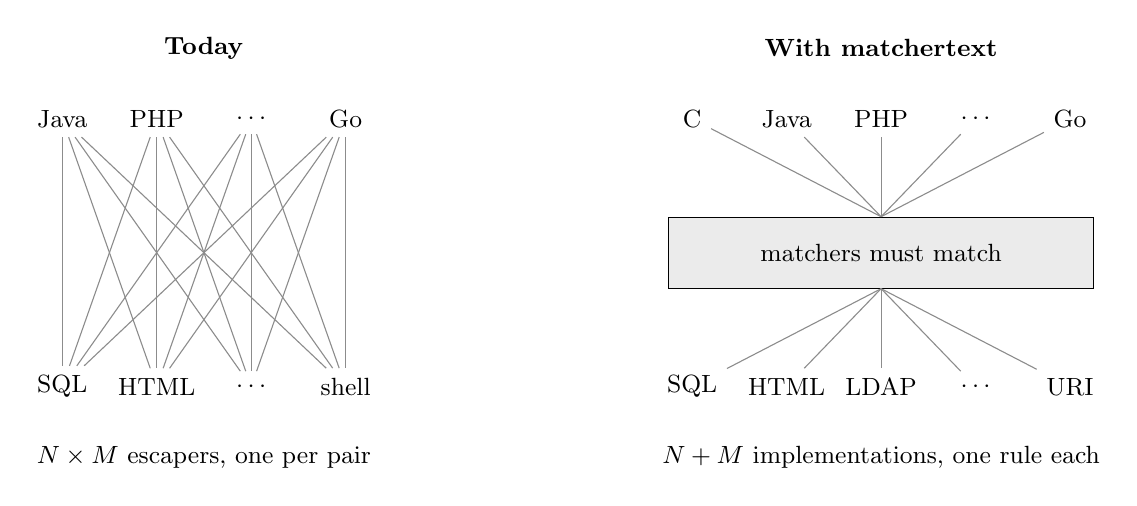
\begin{tikzpicture}[
	lang/.style={font=\small},
	link/.style={draw=black!45, line width=0.4pt},
	waist/.style={draw, fill=black!8, minimum width=5.4cm,
		minimum height=0.9cm, font=\small},
	note/.style={font=\small},
]
\begin{scope}[xshift=-4.3cm]
	\node[note] at (0,2.6) {\textbf{Today}};
	\node[lang] (t1) at (-1.8,1.7) {Java};
	\node[lang] (t2) at (-0.6,1.7) {PHP};
	\node[lang] (t3) at ( 0.6,1.7) {$\cdots$};
	\node[lang] (t4) at ( 1.8,1.7) {Go};
	\node[lang] (s1) at (-1.8,-1.7) {SQL};
	\node[lang] (s2) at (-0.6,-1.7) {HTML};
	\node[lang] (s3) at ( 0.6,-1.7) {$\cdots$};
	\node[lang] (s4) at ( 1.8,-1.7) {shell};
	\foreach \a in {t1,t2,t3,t4}
		\foreach \b in {s1,s2,s3,s4}
			\draw[link] (\a) -- (\b);
	\node[note] at (0,-2.6) {$N \times M$ escapers, one per pair};
\end{scope}
\begin{scope}[xshift=4.3cm]
	\node[note] at (0,2.6) {\textbf{With matchertext}};
	\node[lang] (u1) at (-2.4,1.7) {C};
	\node[lang] (u2) at (-1.2,1.7) {Java};
	\node[lang] (u3) at ( 0.0,1.7) {PHP};
	\node[lang] (u4) at ( 1.2,1.7) {$\cdots$};
	\node[lang] (u5) at ( 2.4,1.7) {Go};
	\node[waist] (w) at (0,0) {matchers must match};
	\node[lang] (v1) at (-2.4,-1.7) {SQL};
	\node[lang] (v2) at (-1.2,-1.7) {HTML};
	\node[lang] (v3) at ( 0.0,-1.7) {LDAP};
	\node[lang] (v4) at ( 1.2,-1.7) {$\cdots$};
	\node[lang] (v5) at ( 2.4,-1.7) {URI};
	\foreach \a in {u1,u2,u3,u4,u5} \draw[link] (\a) -- (w.north);
	\foreach \b in {v1,v2,v3,v4,v5} \draw[link] (w.south) -- (\b);
	\node[note] at (0,-2.6) {$N + M$ implementations, one rule each};
\end{scope}
\end{tikzpicture}
\caption{The narrow waist. Each escaper today is written for one composing
language and one sink, and must model that sink's syntax and track it as it
changes. A rule both sides implement once decouples them, since the rule mentions
neither: any language emitting valid matchertext is compatible with any sink
reading to matcher balance. Not everything passes through the waist, however:
contexts delimited by non-matchers, such as shell separators and CR/LF header
breaks, and sinks that execute their contents by design lie outside it, and
\cref{sec:prevent} measures how much of the recorded landscape that leaves.}
\label{fig:bg:waist}
\end{figure*}

The defenses of \cref{sec:bg:sanitizer} share a shape.
Each is written for one composing language and one sink, and works by knowing the
sink well enough to transform values for it: a Java-to-SQL escaper knows SQL, and
an HTML sanitizer knows the browser's parser closely enough to predict it.
Neither transfers to the other's problem, so the number of defenses to write,
audit, and re-synchronize grows with the product of the two populations.

\Cref{fig:bg:waist} shows the alternative.
A rule that both sides implement once decouples them, because the rule mentions
neither: a language that emits valid matchertext is compatible with every sink
that reads to matcher balance, and such a sink accepts values from every such
language, without either knowing what the other is.
The count falls from $N \times M$ relationships to $N + M$ implementations, which
is the shape the Internet protocol stack takes for the same reason, a waist thin
enough that what sits above and below it can vary independently.

Whether that shape is worth adopting is a security question rather than an
aesthetic one, and it turns on what the shared rule actually guarantees when the
value in the hole is chosen by an attacker.
\Cref{sec:relevance} takes it up.
